\documentclass[a4paper,12pt]{article}
\usepackage[indonesian]{babel}
\usepackage{graphicx}
\usepackage{multirow}
\usepackage{enumitem}
\usepackage{listings}
\usepackage{wrapfig}
\usepackage[T1]{fontenc}
\usepackage{inconsolata}
\usepackage{lipsum}
\usepackage{adjustbox}


\usepackage{color}
\usepackage[table]{xcolor}
\definecolor{lightgray}{rgb}{0.95, 0.95, 0.95}
\definecolor{darkgray}{rgb}{0.4, 0.4, 0.4}
%\definecolor{purple}{rgb}{0.65, 0.12, 0.82}
\definecolor{editorGray}{rgb}{0.95, 0.95, 0.95}
\definecolor{editorOcher}{rgb}{1, 0.5, 0} % #FF7F00 -> rgb(239, 169, 0)
\definecolor{editorGreen}{rgb}{0, 0.5, 0} % #007C00 -> rgb(0, 124, 0)
\definecolor{orange}{rgb}{1,0.45,0.13}		
\definecolor{olive}{rgb}{0.17,0.59,0.20}
\definecolor{brown}{rgb}{0.69,0.31,0.31}
\definecolor{purple}{rgb}{0.38,0.18,0.81}
\definecolor{lightblue}{rgb}{0.1,0.57,0.7}
\definecolor{lightred}{rgb}{1,0.4,0.5}
\usepackage{upquote}
\usepackage{listings}
% CSS
\lstdefinelanguage{CSS}{
  keywords={color,background-image:,margin,padding,font,weight,display,position,top,left,right,bottom,list,style,border,size,white,space,min,width, transition:, transform:, transition-property, transition-duration, transition-timing-function},	
  sensitive=true,
  morecomment=[l]{//},
  morecomment=[s]{/*}{*/},
  morestring=[b]',
  morestring=[b]",
  alsoletter={:},
  alsodigit={-}
}

% JavaScript
\lstdefinelanguage{JavaScript}{
  morekeywords={typeof, new, true, false, catch, function, return, null, catch, switch, var, if, in, while, do, else, case, break},
  morecomment=[s]{/*}{*/},
  morecomment=[l]//,
  morestring=[b]",
  morestring=[b]'
}

\lstdefinelanguage{HTML5}{
  language=html,
  sensitive=true,	
  alsoletter={<>=-},	
  morecomment=[s]{<!-}{-->},
  tag=[s],
  otherkeywords={
  % General
  >,
  % Standard tags
	<!DOCTYPE,
  </html, <html, <head, <title, </title, <style, </style, <link, </head, <meta, />,
	% body
	</body, <body,
	% Divs
	</div, <div, </div>, 
	% Paragraphs
	</p, <p, </p>,
	% scripts
	</script, <script,
  % More tags...
  <canvas, /canvas>, <svg, <rect, <animateTransform, </rect>, </svg>, <video, <source, <iframe, </iframe>, </video>, <image, </image>, <header, </header, <article, </article
  },
  ndkeywords={
  % General
  =,
  % HTML attributes
  charset=, src=, id=, width=, height=, style=, type=, rel=, href=,
  % SVG attributes
  fill=, attributeName=, begin=, dur=, from=, to=, poster=, controls=, x=, y=, repeatCount=, xlink:href=,
  % properties
  margin:, padding:, background-image:, border:, top:, left:, position:, width:, height:, margin-top:, margin-bottom:, font-size:, line-height:,
	% CSS3 properties
  transform:, -moz-transform:, -webkit-transform:,
  animation:, -webkit-animation:,
  transition:,  transition-duration:, transition-property:, transition-timing-function:,
  }
}

\lstdefinestyle{htmlcssjs} {%
  % General design
%  backgroundcolor=\color{editorGray},
  basicstyle={\footnotesize\ttfamily},   
  frame=b,
  % line-numbers
  xleftmargin={0.75cm},
  numbers=left,
  stepnumber=1,
  firstnumber=1,
  numberfirstline=true,	
  % Code design
  identifierstyle=\color{black},
  keywordstyle=\color{blue}\bfseries,
  ndkeywordstyle=\color{editorGreen}\bfseries,
  stringstyle=\color{editorOcher}\ttfamily,
  commentstyle=\color{brown}\ttfamily,
  % Code
  language=HTML5,
  alsolanguage=JavaScript,
  alsodigit={.:;},	
  tabsize=2,
  showtabs=false,
  showspaces=false,
  showstringspaces=false,
  extendedchars=true,
  breaklines=true,
}
\lstset{
    frame=single,
    breaklines=true,
}
%

\graphicspath{ {./img/} }
\begin{document}
\title{ {\Large Laporan Praktikum}\\ Pemrograman Web Client\\{\Large Pertemuan 3}}

\author{Aldzikri Dwijayanto Prathama 
	\\195410189
	\\Informatika}
\makeatletter
\begin{titlepage}
	\begin{center}
		{\huge \bfseries \@title }\\[14ex]
		
\includegraphics[scale=.8]{logo}\\[4ex]
		{\large \@author}\\[12ex]
		{\large \bfseries {SEKOLAH TINGGI MANAJEMEN INFORMATIKA DAN KOMPUTER
				AKAKOM YOGYAKARTA}}
	\end{center}


%{\large \@date} 
\end{titlepage}
\makeatother
%\maketitle
\newpage
\tableofcontents
\newpage
\section{Tujuan}
\begin{enumerate}
    \item Menuliskan CSS sesuai aturan (properti dan nilai)
    \item Menuliskan selektor tag
    \item Menuliskan selektor id
    \item Menuliskan selektor class
    \item Menuliskan script internal style
    \item Menuliskan script eksternal style
    \item Menuliskan inline style
\end{enumerate}
\section{Dasar Teori}
CSS (Cascading Style Sheets) adalah script program yang digunakan untuk mengatur
tampilan website, misalnya warna body , jenis serta ukuran font, layout website.
Perintah html hanya mampu mengatur tampilan untuk satu halaman site sedangkan CSS
mampu mengontrol tampilan banyak halaman sekaligus. CSS tidak dikategorikan sebagai
bahasa pemrograman karena di dalamnya tidak ada struktur kontrol (percabangan,
perulangan, array dll). CSS dapat ditambahkan ke dalam HTML dengan 3 cara:
\begin{enumerate}[label=\alph*.]
    \item inline : melalui atribut “style” pada elemen Html
    \item internal : melalui tag <style> yang diletakkan di dalam tag <Head>
    \item eksternal : CSS disimpan pada sebuah file tersendiri dengan ekstensi *.css
\end{enumerate}

\newpage

\section{Pembahasan}
\subsection{Praktik}
\subsubsection{Praktik 1}
\begin{lstlisting}
<!DOCTYPE html>
<html>
    <head>
        <style>
            body{
                background-color: linen;
            }
            h1 {
                color: green;
                margin-left:40px;
            }
            p{
                color: red;
                margin-left:20px;
            }
        </style>
    </head>
    <body>
        <h1>STMIK AKAKOM</h1>
        <p>Alamat: Jl.Janti no.143, 
        Jaranan, Karang Jambe, 
        Kec. Banguntapan, Bantul, DIY 55918</p>

        <p>Telepon: (0274) 486664</p>
    </body>
</html>
\end{lstlisting}
Pada dokumen html tersebut, terdapat CSS dengan jenis internal, karena script css tersebut 
dimasukkan ke dalam tag <head>. Dari syntax css di atas dari selektornya dikeathui elemen 
yang akan diatur adalah elemen body yang diatur backgroundnya menjadi warna linen. Dan elemen 
h1 dan p diatur warna dan marginnya. Jika dibuka di browser tampilannya seperti berikut:
\begin{center}
    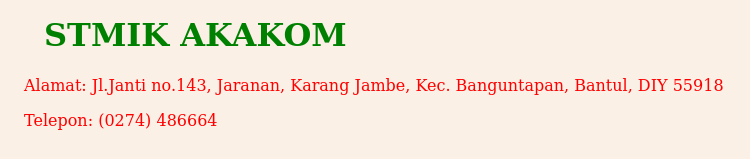
\includegraphics[width=\linewidth]{1.png}
\end{center}

\subsubsection{Praktik 2}
\begin{lstlisting}
<!DOCTYPE html>
<html>
    <body>
    <h1 style="color:blue;text-align:center;">STMIK AKAKOM</h1>
    <p style="color:red;text-align:center">Telepon: (0274) 486664</p>
    </body>
</html>
\end{lstlisting}

Dokumen html tersebut memiliki CSS secara inline, karena dimasukkan langsung di elemen yang
akan diatur tampilannya.
\begin{center}
    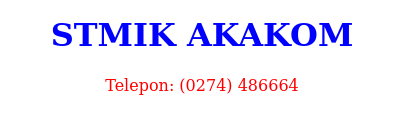
\includegraphics[width=\linewidth]{2.png}
\end{center}

\subsubsection{Praktik 3}
Pada praktik 3 dibuat dokumen html, yang script CSS nya terpisah, Pertama buat file dengan nama desainku.css, dengan isi sebagai berikut:
\begin{lstlisting}
body {
    background-color: lightblue;
}
h1 {
    color: navy;
    margin-left: 20px;
}
\end{lstlisting}
File css tersebut akan mengatur warna background menjadi warna lightblue, dan elemen h1 diatur menjadi warna navy, dan margin kiri 20 pixel.\\
Setelah itu buat file html dengan nama eksternalCSS.html, isi seperti ini:
\begin{lstlisting}
<!DOCTYPE html>
<html>
    <head>
        <link rel="stylesheet" type="text/css" href="desainku.css">
    </head>
    <body>
        <h1>STMIK AKAKOM</h1>
        <p>Telepon: (0274) 486664</p>
    </body>
</html>
\end{lstlisting}
Pada tag head didalamnya terdapat tag link, yang akan menginstruksikan browser untuk memuat file desainku.css dan menerapkan pengaturan yang ditentukan ke dokumen html tersebut.
\begin{center}
    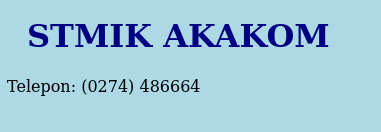
\includegraphics[width=\linewidth]{3.png}
\end{center}

\subsubsection{Praktik 4}
Praktik 4 adalah membuat css internal yang menggunakan id css
\begin{lstlisting}
<!DOCTYPE html>
<html>
    <head>
        <style>
            #kampus {
            text-align: center;
            color: red;
            }
        </style>
    </head>
    <body>
        <p id="kampus">STMIK AKAKOM</p>
        <p>Telepon: (0274) 486664</p>
    </body>
</html>
\end{lstlisting}
Script CSS yang digunakan ditulis pada tag style, di dalam tag head, tanda pagar(\#) menandakan bahwa script CSS tersbut berbentuk ID. Untuk menggunakan CSS ini kita perlu 
menyertakannya ke dalam tag yang ingin kita atur tampilannya.\\
Untuk dokumen html di atas yang di atur adalah tag p yang pertama. Karena ID CSS hanya bisa 
panggil sekali, maka kita hanya bisa menggunakannya pada salah satu tag saja.
\begin{center}
    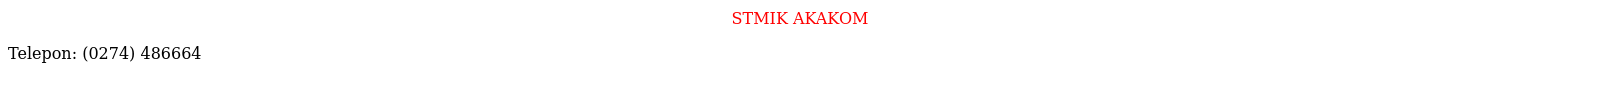
\includegraphics[scale=0.4]{4.png}
\end{center}

\subsubsection{Praktik 5}
Untuk praktik 5, adalah membuat css internal yang menggunakan class.
\begin{lstlisting}
<!DOCTYPE html>
<html>
    <head>
        <style>
            .center {
            text-align: center;
            color: red;
            }
        </style>
    </head>
    <body>
        <h1 class="center">STMIK AKAKOM</h1>
        <p class="center">Telepon: (0274) 486664</p>
    </body>
</html>
\end{lstlisting}
Script CSS yang digunakan ditulis pada tag style, di dalam tag head, tanda titik(.) menandakan bahwa script CSS tersebut berbentuk Class. Untuk menggunakan CSS ini kita perlu 
menyertakannya ke dalam tag yang ingin kita atur tampilannya.\\
Untuk dokumen html di atas yang di atur adalah tag h1 dan p. Karena Class CSS bisa 
dipanggil berulangkali, maka kita bisa menggunakannya pada beberapa tag.
\begin{center}
    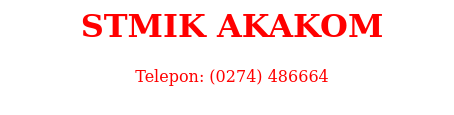
\includegraphics[width=\linewidth]{5.png}
\end{center}

\newpage

\subsection{Latihan}
\subsubsection{Latihan 1}
Untuk latihan 1, adalah mengubah praktik 4 agar CSS menjadi eksternal. Caranya cukup dengan 
memindahkan CSS di dalam tag style ke file baru dengan ekstensi css. Dan memanggilnya 
dengan tag link.\\
Isi dari file CSS untuk Latihan 1 sebagai berikut:
\begin{lstlisting}
#kampus {
text-align: center;
color: red;
}
\end{lstlisting}
Sedangkan untuk file htmlnya seperti berikut:
\begin{lstlisting}
<!DOCTYPE html>
<html>
    <head>
        <link rel="stylesheet" type="text/css" href="latihan1.css">
    </head>
    <body>
        <p id="kampus">STMIK AKAKOM</p>
        <p>Telepon: (0274) 486664</p>
    </body>
</html>
\end{lstlisting}
\begin{center}
    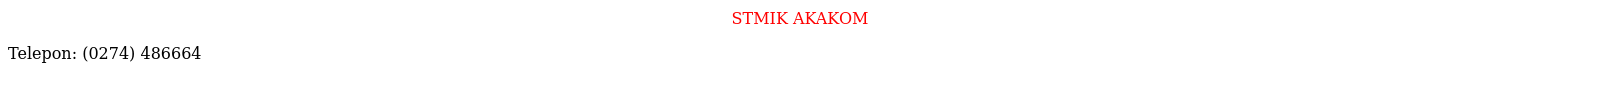
\includegraphics[scale=0.4]{4.png}
\end{center}

\subsubsection{Latihan 2}
Sama dengan latihan sebelumnya, yaitu mengubah Praktik 5 agar memiliki CSS eksternal. Caranya 
pun sama dengan praktik 1.\\
Isi dari file css:
\begin{lstlisting}
.center {
text-align: center;
color: red;
}
\end{lstlisting}
Isi file html:
\begin{lstlisting}
<!DOCTYPE html>
<html>
    <head>
        <link rel="stylesheet" type="text/css" href="latihan2.css">
    </head>
    <body>
        <h1 class="center">STMIK AKAKOM</h1>
        <p class="center">Telepon: (0274) 486664</p>
    </body>
</html>
\end{lstlisting}
\begin{center}
    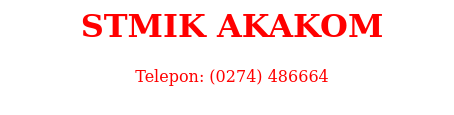
\includegraphics[width=\linewidth]{5.png}
\end{center}

\newpage

\subsection{Tugas}
Untuk tugas adalah merubah salah satu praktik di atas yang belum diubah CSS-nya menjadi CSS eksternal. Untuk praktik 1 agar CSS-nya menjadi eksternal kita perlu memindahkan bagian CSS ke file 
baru berekstensi CSS.
\begin{lstlisting}
body{
    background-color: linen;
}
h1 {
    color: green;
    margin-left:40px;
}
p{
    color: red;
    margin-left:20px;
}
\end{lstlisting}
Dan memanggilnya menggunakan tag link di file html.
\begin{lstlisting}
<!DOCTYPE html>
<html>
    <head>
        <link rel="stylesheet" type="text/css" href="Tugas1.css">
    </head>
    <body>
        <h1>STMIK AKAKOM</h1>
        <p>Alamat: Jl.Janti no.143, 
        Jaranan, Karang Jambe, 
        Kec. Banguntapan, Bantul, DIY 55918</p>

        <p>Telepon: (0274) 486664</p>
    </body>
</html>
\end{lstlisting}
Tampilan saat dibuka di browser.
\begin{center}
    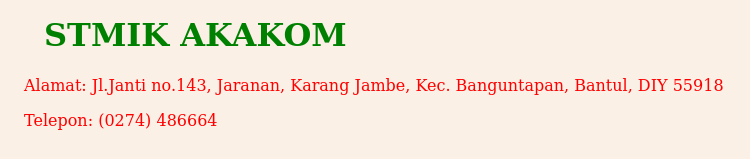
\includegraphics[width=\linewidth]{1.png}
\end{center}

\newpage
\section{Kesimpulan}
Setelah praktik ini, mahasiswa mampu menuliskan CSS sesuai aturan (properti dan nilai), selektor tag, selektor id, selektor class, script internal style, script eksternal style, dan inline style
\end{document}
